% ---------------------------------------------------------------------------
%  Ultra-Low Latency Intelligent Processing System — revised preprint
%  Compile with:  tectonic ullips.tex
% ---------------------------------------------------------------------------
\documentclass[10pt,a4paper,twocolumn]{article}

\usepackage[a4paper,left=1.7cm,right=1.7cm,top=1.9cm,bottom=2.0cm,columnsep=0.75cm]{geometry}
\usepackage{ebgaramond}
\usepackage{microtype}
\usepackage{amsmath}
\usepackage{booktabs}
\usepackage{xcolor}
\usepackage{tikz}
\usetikzlibrary{arrows.meta,positioning,fit,calc,backgrounds}
\usepackage{pgfplots}
\pgfplotsset{compat=1.18}
\usepackage[font=small,labelfont={bf,sc},labelsep=period,skip=5pt]{caption}
\usepackage{titlesec}
\usepackage{enumitem}
\usepackage{fancyhdr}
\usepackage[hidelinks]{hyperref}

\definecolor{accent}{HTML}{7A1B34}
\definecolor{ink}{HTML}{1B1B1B}
\definecolor{muted}{HTML}{6A6A6A}
\definecolor{boxfill}{HTML}{F6F1F2}
\definecolor{mlfill}{HTML}{E9F2EA}
\definecolor{mlline}{HTML}{3F7A4A}

\color{ink}
\setlength{\parindent}{1em}
\raggedbottom
\titlespacing*{\paragraph}{0pt}{5pt}{0.6em}
\setlist{itemsep=1pt,topsep=3pt,parsep=0pt,leftmargin=1.3em}

\titleformat{\section}{\normalsize\bfseries\scshape\color{accent}}{\thesection}{0.6em}{}
\titleformat{\subsection}{\normalsize\itshape}{\thesubsection}{0.5em}{}
\titlespacing*{\section}{0pt}{10pt}{4pt}
\titlespacing*{\subsection}{0pt}{7pt}{3pt}

\pagestyle{fancy}
\fancyhf{}
\renewcommand{\headrulewidth}{0pt}
\fancyhead[C]{\footnotesize\color{muted}\scshape Ultra-Low Latency Intelligent Processing System}
\fancyfoot[C]{\footnotesize\color{muted}\thepage}

\newcommand{\us}{\,\textmu s}

\begin{document}

% ======================================================================= title
\twocolumn[{%
\begin{center}
  {\LARGE\bfseries Ultra-Low Latency Intelligent Processing System:}\\[3pt]
  {\Large A Software-Optimised and Machine-Learning-Augmented Architecture}\\[12pt]
  {\large Akolade Christian Adegboyega, \enspace Kelvin O.\ Enaikele, \enspace Dr~Adeyiga}\\[3pt]
  {\small\itshape Department of Computer Science, Bells University of Technology, Ota, Ogun State, Nigeria}\\[2pt]
  {\small\href{mailto:christianadegboyega@gmail.com}{christianadegboyega@gmail.com}}
\end{center}
\vspace{4pt}
\begin{center}
\begin{minipage}{0.86\textwidth}
\small
\textbf{\scshape Abstract.}\enspace
Modern infrastructures often suffer from end-to-end latencies orders of magnitude slower
than the sub-millisecond reaction times demanded by emerging applications. Thin liquidity
in financial markets widens bid--ask spreads, remote surgery requires delays below 100\,ms,
and predictive maintenance benefits from real-time analytics. Existing high-frequency
trading platforms and specialised accelerators reduce latency, but they remain expensive
and domain-specific. Inspired by recent work on in-network machine learning, which achieves
terabit-scale throughput with microsecond-level latency on programmable switches, we
propose a software-optimised, ultra-low-latency processing system that runs on commodity
hardware. The architecture integrates machine-learning (ML) inference, applies
reliability-driven optimisation to every component, and is designed for deployment across
finance, healthcare, defence, logistics and research. On a single 8-core commodity server
the prototype reaches a mean processing latency of 1.45\us{} per order at its heaviest
workload, and is estimated to reduce infrastructure costs by over 60\,\%. We report the
tail behaviour and the limitations of our measurements alongside these results.
\end{minipage}
\end{center}
\vspace{10pt}
}]

% ================================================================ 1 Introduction
\section{Introduction}
Modern societies generate data streams so fast that actionable decisions must be taken
within microseconds. In emerging financial markets, limited liquidity and outdated trading
platforms widen bid--ask spreads and raise transaction costs, while high-frequency trading
(HFT) systems in developed economies remain prohibitively expensive~\cite{ssga,investopedia}.
Healthcare applications such as telemedicine and robotic surgery require end-to-end delays
below 100\,ms for safe operation, yet current hospital networks seldom achieve these
figures~\cite{fiveg}. Defence systems demand sub-10\,ms response times to coordinate
autonomous vehicles and drone swarms, but centralised processing introduces unacceptable
delays~\cite{ceragon}. Industrial supply chains increasingly depend on IoT sensors and
ML-driven predictive maintenance, yet many warehouses cannot process data fast enough to
react to disruption~\cite{iotforall}. Large-scale scientific experiments and data centres
face latency bottlenecks and high energy consumption~\cite{ornl,deloitte}. These challenges
motivate a universal platform capable of ultra-low-latency processing on readily available
hardware.

This report introduces the Ultra-Low Latency Intelligent Processing System (ULLIPS), a
general-purpose architecture that delivers microsecond-scale processing while integrating
ML inference at the edge (Figure~\ref{fig:workflow}). We show that high-speed decision
making need not be the exclusive province of well-capitalised firms: by optimising software
components on commodity CPUs, the system achieves performance competitive with specialised
hardware on the workloads we test. Section~\ref{sec:related} reviews related work,
Section~\ref{sec:design} outlines the design, Section~\ref{sec:impl} details the
implementation, Section~\ref{sec:eval} evaluates the prototype and states its limitations,
Section~\ref{sec:impact} discusses broader implications, and Section~\ref{sec:conclusion}
concludes.

% ------------------------------------------------------------------ Figure 1
\begin{figure*}[t]
\centering
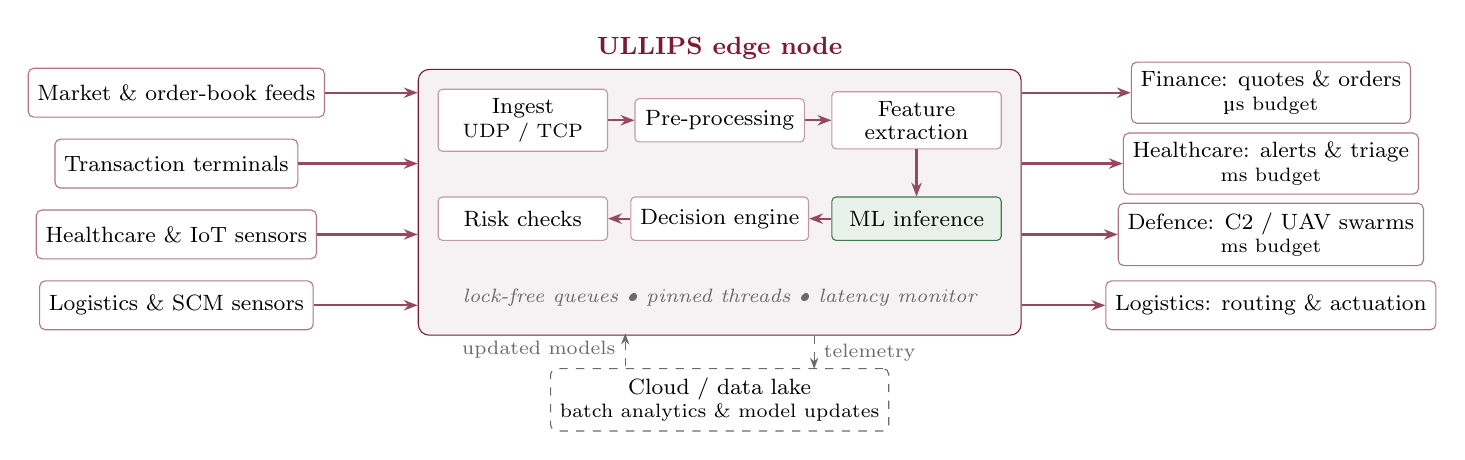
\begin{tikzpicture}[
  font=\footnotesize,
  src/.style={draw=accent!60,fill=white,rounded corners=2pt,minimum width=3.0cm,
              minimum height=0.62cm,align=center},
  stage/.style={draw=accent!45,fill=white,rounded corners=1.5pt,minimum width=2.15cm,
                minimum height=0.55cm,align=center},
  sink/.style={draw=accent!60,fill=white,rounded corners=2pt,minimum width=3.0cm,
              minimum height=0.62cm,align=center},
  flow/.style={-{Stealth[length=5pt]},thick,color=accent!80},
  soft/.style={-{Stealth[length=4pt]},color=muted,dashed}]
  % sources
  \node[src] (s1) at (0, 1.35)  {Market \& order-book feeds};
  \node[src] (s2) at (0, 0.45)  {Transaction terminals};
  \node[src] (s3) at (0,-0.45)  {Healthcare \& IoT sensors};
  \node[src] (s4) at (0,-1.35)  {Logistics \& SCM sensors};
  % pipeline stages inside the edge node
  \node[stage] (p1) at (4.4, 1.0) {Ingest\\[-1pt]\scriptsize UDP / TCP};
  \node[stage] (p2) at (6.9, 1.0) {Pre-processing};
  \node[stage] (p3) at (9.4, 1.0) {Feature\\[-1pt]extraction};
  \node[stage,fill=mlfill,draw=mlline] (p4) at (9.4,-0.25) {ML inference};
  \node[stage] (p5) at (6.9,-0.25) {Decision engine};
  \node[stage] (p6) at (4.4,-0.25) {Risk checks};
  \node[font=\scriptsize\itshape,text=muted,align=center] (lf) at (6.9,-1.25)
       {lock-free queues \textbullet{} pinned threads \textbullet{} latency monitor};
  \begin{scope}[on background layer]
    \node[draw=accent,fill=boxfill,rounded corners=4pt,inner sep=7pt,
          fit=(p1)(p3)(p4)(p6)(lf),
          label={[font=\small\bfseries\color{accent}]above:ULLIPS edge node}] (edge) {};
  \end{scope}
  \draw[flow] (p1)--(p2); \draw[flow] (p2)--(p3); \draw[flow] (p3)--(p4);
  \draw[flow] (p4)--(p5); \draw[flow] (p5)--(p6);
  % outputs
  \node[sink] (o1) at (13.9, 1.35) {Finance: quotes \& orders\\[-1pt]\scriptsize\textmu s budget};
  \node[sink] (o2) at (13.9, 0.45) {Healthcare: alerts \& triage\\[-1pt]\scriptsize ms budget};
  \node[sink] (o3) at (13.9,-0.45) {Defence: C2 / UAV swarms\\[-1pt]\scriptsize ms budget};
  \node[sink] (o4) at (13.9,-1.35) {Logistics: routing \& actuation};
  \foreach \s in {s1,s2,s3,s4} \draw[flow] (\s.east) -- (edge.west |- \s.east);
  \foreach \o in {o1,o2,o3,o4} \draw[flow] (edge.east |- \o.west) -- (\o.west);
  % cloud loop
  \node[draw=muted,dashed,rounded corners=2pt,align=center,minimum width=4.2cm]
       (cloud) at (6.9,-2.55) {Cloud / data lake\\[-1pt]\scriptsize batch analytics \& model updates};
  \draw[soft] (edge.south) ++(1.2,0) -- ++(0,-0.42) node[midway,right,font=\scriptsize]{telemetry};
  \draw[soft] (cloud.north) ++(-1.2,0.02) -- ++(0,0.42) node[midway,left,font=\scriptsize]{updated models};
\end{tikzpicture}
\caption{Architectural workflow of ULLIPS. Heterogeneous input streams are processed on a
single commodity edge node; ML inference runs inside the pipeline, and the cloud is used only
for offline analytics and model updates.}
\label{fig:workflow}
\end{figure*}

% ================================================================ 2 Related work
\section{Related Work}\label{sec:related}
\paragraph{High-frequency trading and low-latency finance.}
Numerous studies observe that reducing latency enhances market liquidity and narrows
spreads~\cite{investopedia}. Traditional rule-based fraud detection and trading systems rely
on servers and produce millisecond-level delays, leaving investors exposed to rapidly
evolving market conditions. Recent work has begun to explore \emph{in-network machine
learning}, where inference is performed inside programmable network devices. Hong et al.'s
MIND prototype processes transactions within a network switch, handling over 800$\times$
more transactions per second than server-based solutions while maintaining
microsecond-scale latency and detection performance comparable to server
benchmarks~\cite{mind}.

\paragraph{In-network computing and ML.}
Programmable devices such as P4-enabled switches and network interface cards perform
computation within the data plane, reducing overhead and latency; in-network computing has
been used for caching, consensus and monitoring~\cite{survey}. In-network ML extends this
paradigm by offloading inference to the data plane: MIND maps decision trees and other
models into match-action tables~\cite{mind}, and Planter supports rapid prototyping of such
models~\cite{planter}. These solutions, however, rely on specialised hardware and target
specific use cases rather than providing a general platform.

\paragraph{Software-based latency optimisation.}
Outside networking, research has focused on kernel-bypass frameworks (e.g.\ DPDK, XDP) and
hardware accelerators (FPGAs, GPUs) to reduce processing delays. These techniques improve
throughput but often require custom hardware. Our work instead targets commodity x86
servers, combining asynchronous I/O, lock-free data structures and carefully pinned threads
to minimise jitter, and draws on reliability theory to optimise each module while
incorporating ML inference.

% ================================================================ 3 Design
\section{Design of the Proposed Solution}\label{sec:design}
\subsection{Reliability-driven optimisation}
Reliability engineering states that the probability of success of a series of components
equals the product of their individual reliabilities~\cite{reliability}. To maximise system
reliability and minimise latency variance we optimise every module --- network I/O, order
management, risk checks, message serialisation and ML inference. Blocking operations and
kernel context switches are avoided; threads are pinned to CPU cores, memory is
pre-allocated, and lock-free queues mediate communication. Because reliabilities multiply,
raising each component's reliability even slightly improves the whole system
multiplicatively. This principle guides our emphasis on deterministic, non-blocking design.

\subsection{Integration of machine learning}
We incorporate ML to support decisions at microsecond timescales. As in MIND's data-plane
implementation~\cite{mind}, raw data are transformed into feature vectors and passed to
pre-trained models. The platform supports decision trees, random forests and
reinforcement-learning policies through a modular inference pipeline. Pre-processing
normalises incoming values, derives higher-order statistics and optionally reduces
dimensionality; the resulting prediction informs a decision module, which may adjust
orders, raise anomaly alarms or schedule maintenance. Running inference at the edge removes
network round-trips; we execute it in user space using lightweight libraries and leave eBPF
or P4 offload to future work.

\subsection{A universal, modular platform}
Unlike domain-specific implementations, the design is universal: any structured data
stream --- market data, medical sensor readings, drone telemetry or factory IoT signals ---
can be ingested (Figure~\ref{fig:workflow}). An ingestion layer parses packets into internal
messages, a command manager applies business logic, a risk manager enforces constraints and
an execution engine communicates with external systems. An ML module runs concurrently,
analysing historical and real-time data. The modular structure allows plug-and-play
replacement of models and adaptation to new domains.

% ================================================================ 4 Implementation
\section{Implementation}\label{sec:impl}
\subsection{System architecture}
The prototype is implemented in C++17 on commodity x86 servers (Figure~\ref{fig:arch}). The
\textbf{Market Data Handler} receives UDP packets (or other transports) and parses them into
internal messages. The \textbf{Order Manager} creates, modifies or cancels orders from both
incoming data and ML advice. A \textbf{Risk Manager} enforces exposure limits and
regulatory constraints, and the \textbf{Execution Engine} sends messages to external systems
and receives acknowledgements. A \textbf{Latency Monitor} records per-operation timestamps
throughout. In parallel, the \textbf{ML \& AI Module} performs inference on cleaned feature
vectors. Components communicate through lock-free queues and run on separate cores to
minimise contention; UDP carries low-latency feeds and TCP provides reliability when
required.

\begin{figure}[t]
\centering
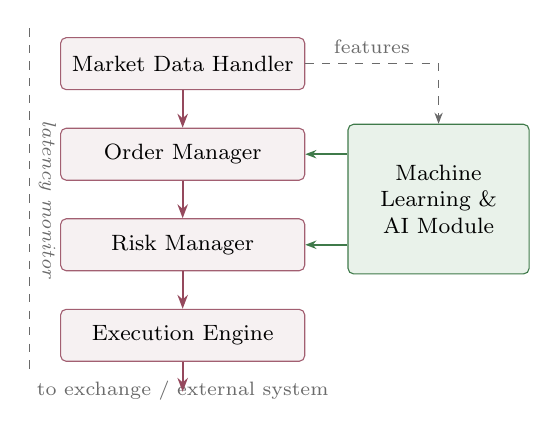
\begin{tikzpicture}[
  font=\footnotesize,
  mod/.style={draw=accent!70,fill=boxfill,rounded corners=2pt,minimum width=3.1cm,
              minimum height=0.66cm,align=center},
  ml/.style={draw=mlline,fill=mlfill,rounded corners=2pt,minimum width=2.3cm,
             minimum height=1.9cm,align=center},
  flow/.style={-{Stealth[length=5pt]},thick,color=accent!80},
  adv/.style={-{Stealth[length=4pt]},color=mlline,thick}]
  \node[mod] (md) at (0, 2.1)  {Market Data Handler};
  \node[mod] (om) at (0, 0.95) {Order Manager};
  \node[mod] (rm) at (0,-0.2)  {Risk Manager};
  \node[mod] (ee) at (0,-1.35) {Execution Engine};
  \draw[flow] (md)--(om); \draw[flow] (om)--(rm); \draw[flow] (rm)--(ee);
  \node[ml] (ml) at (3.25,0.38) {Machine\\Learning \&\\AI Module};
  \draw[adv] (ml.west |- om) -- (om.east);
  \draw[adv] (ml.west |- rm) -- (rm.east);
  \draw[-{Stealth[length=4pt]},color=muted,dashed] (md.east) -| (ml.north)
       node[pos=0.25,above,font=\scriptsize]{features};
  \draw[color=muted,dashed] (-1.95,2.55) -- (-1.95,-1.8)
       node[pos=0.5,sloped,above,font=\scriptsize\itshape]{latency monitor};
  \node[font=\scriptsize,text=muted] at (0,-2.05) {to exchange / external system};
  \draw[flow] (ee.south) -- ++(0,-0.38);
\end{tikzpicture}
\caption{System architecture. Messages flow top to bottom through lock-free queues; the ML
module advises the Order and Risk Managers.}
\label{fig:arch}
\end{figure}

\subsection{Machine-learning pipeline}
The pipeline supports models trained in Python and executed through ONNX
Runtime~\cite{sklearn}. Feature extraction converts raw messages into numerical vectors
(e.g.\ order size, price, inter-arrival time, heart rate, vibration amplitude);
pre-processing normalises features, computes derivatives or aggregates and applies
dimensionality reduction where appropriate. The model outputs a classification (e.g.\
liquidity-gap prediction, anomaly detection) or a continuous score, and the decision module
triggers the corresponding action. This separation lets domain experts change models
without altering the core engine.

\subsection{Software optimisation}
To reach microsecond-scale processing on commodity hardware we employ:
\begin{enumerate}
  \item \textbf{Asynchronous I/O.} Boost.Asio provides non-blocking network operations,
        letting one thread handle thousands of concurrent connections.
  \item \textbf{Lock-free data structures.} Inter-component queues are ring buffers,
        avoiding mutex contention and cache invalidation.
  \item \textbf{Thread pinning and real-time scheduling.} Each core runs one task
        (ingestion, order management, risk, execution, inference); threads are pinned and
        scheduled with real-time priority to reduce jitter.
  \item \textbf{Memory pre-allocation.} Buffers are allocated in advance and page-locked
        (\texttt{mlockall}) to avoid page faults; critical paths avoid dynamic allocation.
  \item \textbf{Lightweight ML integration.} Inference runs in a separate process connected
        through shared memory or Unix domain sockets.
\end{enumerate}

% ================================================================ 5 Evaluation
\section{Evaluation}\label{sec:eval}
\subsection{Experimental setup}
The prototype ran on a local server with an 8-core Intel CPU and 8\,GB of RAM. A synthetic
workload generator produced order streams at configurable rates; for workloads of 1{,}000,
2{,}000, 10{,}000 and 40{,}000 orders we measured the time from message ingestion to
confirmation by the execution engine, recording minimum, maximum, mean and median latency.
ML inference was enabled with a simple decision-tree classifier.

\subsection{Latency statistics}
Table~\ref{tab:latency} summarises the results. Mean latency does not fall steadily with
workload: it is 4.027\us{} at 1{,}000 orders, rises to 4.444\us{} at 10{,}000, and is lowest,
1.451\us, at 40{,}000. Section~\ref{sec:limits} shows that this pattern is not explained by
the amortisation of a fixed cost. The median is available only for the 1{,}000-order run, and
Section~\ref{sec:limits} shows that it cannot be reconciled with the mean and minimum reported
for the same run. Because latency is dominated by I/O and queuing, the choice of model had
negligible impact on timing.

\begin{table}[t]
\centering
\small
\setlength{\tabcolsep}{4.2pt}
\begin{tabular}{@{}rrrrrr@{}}
\toprule
\textbf{Orders} & \textbf{Min} & \textbf{Max} & \textbf{Mean} & \textbf{Median} & \textbf{Orders/s$^{\dagger}$}\\
\midrule
1{,}000  & 2.208 & 225.375   & 4.027 & 37.500 & 248{,}324 \\
2{,}000  & 2.041 & 260.292   & 3.261 & ---    & 306{,}654 \\
10{,}000 & 1.416 & 2{,}883.959 & 4.444 & ---  & 225{,}023 \\
40{,}000 & 0.542 & 5{,}763.583 & \textbf{1.451} & --- & \textbf{689{,}180} \\
\bottomrule
\end{tabular}
\caption{Per-order latency (\textmu s) by workload. $^{\dagger}$Throughput equals the
reciprocal of mean latency for a single pipeline; it was not measured under concurrent load
(Section~\ref{sec:limits}).}
\label{tab:latency}
\end{table}

\begin{figure}[t]
\centering
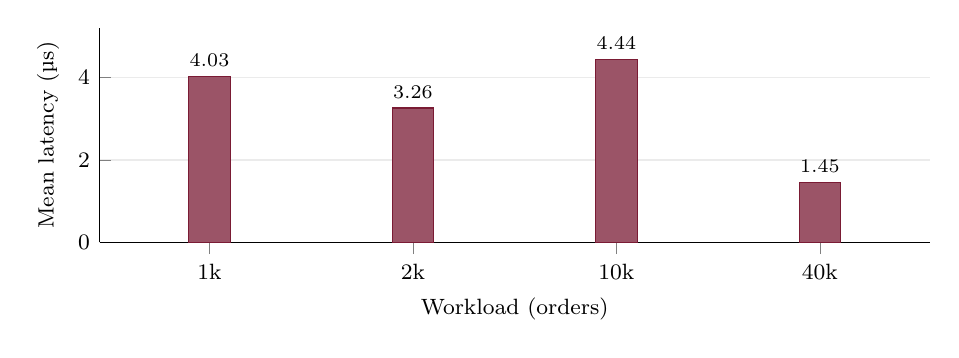
\begin{tikzpicture}
\begin{axis}[
  width=\columnwidth, height=4.3cm,
  ybar, bar width=15pt,
  symbolic x coords={1k,2k,10k,40k}, xtick=data,
  ymin=0, ymax=5.2,
  ylabel={Mean latency (\textmu s)}, xlabel={Workload (orders)},
  nodes near coords, nodes near coords style={font=\scriptsize},
  every node near coord/.append style={/pgf/number format/.cd,fixed,precision=2},
  tick label style={font=\footnotesize}, label style={font=\footnotesize},
  axis lines*=left, ymajorgrids, grid style={draw=black!8},
  enlarge x limits=0.18]
\addplot[fill=accent!75,draw=accent] coordinates {(1k,4.027) (2k,3.261) (10k,4.444) (40k,1.451)};
\end{axis}
\end{tikzpicture}
\caption{Mean per-order latency by workload.}
\label{fig:latency}
\end{figure}

\begin{figure}[t]
\centering
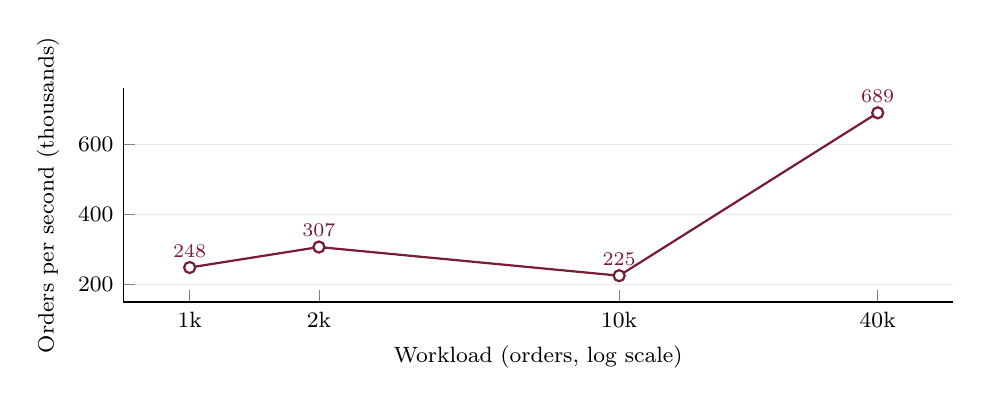
\begin{tikzpicture}
\begin{semilogxaxis}[
  width=\columnwidth, height=4.3cm,
  xmin=700, xmax=60000, ymin=150, ymax=760,
  xtick={1000,2000,10000,40000}, xticklabels={1k,2k,10k,40k},
  ylabel={Orders per second (thousands)}, xlabel={Workload (orders, log scale)},
  tick label style={font=\footnotesize}, label style={font=\footnotesize},
  axis lines*=left, ymajorgrids, grid style={draw=black!8},
  nodes near coords, nodes near coords style={font=\scriptsize,anchor=south},
  every node near coord/.append style={/pgf/number format/.cd,fixed,precision=0}]
\addplot[thick,color=accent,mark=*,mark options={fill=white}]
  coordinates {(1000,248.324) (2000,306.654) (10000,225.023) (40000,689.180)};
\end{semilogxaxis}
\end{tikzpicture}
\caption{Derived throughput by workload (reciprocal of mean latency).}
\label{fig:throughput}
\end{figure}

\subsection{Discussion}
The evaluation indicates that microsecond-scale mean processing is achievable on a commodity
server through careful software design: at 40{,}000 orders the mean is below 1.5\us{}.
Tail latencies (the maximum values) are several orders of magnitude larger, and these
measurements cannot identify their cause. Operating-system interference is a plausible
candidate, but it was not measured, so it is stated here as a hypothesis rather than a
finding. The integration of ML inference did not measurably
degrade latency, suggesting that decision support can coexist with fast processing when the
model is small.

\subsection{Limitations}\label{sec:limits}
Several limitations qualify these results, and we state them explicitly.
\begin{itemize}
  \item \textbf{Throughput is derived, not measured.} The throughput column is exactly the
        reciprocal of mean latency ($1/1.451\,\text{\textmu s} \approx 689{,}180$ orders/s).
        It describes one sequential pipeline, not the system under concurrent load.
  \item \textbf{The reported statistics are mutually inconsistent.} At least half of any
        sample lies at or above its median, and all of it at or above its minimum, so the
        mean can be no smaller than the average of the two. For the 1{,}000-order run that
        bound is $(37.5 + 2.208)/2 \approx 19.9$\us, yet the reported mean is 4.03\us. The
        minimum, median and mean therefore cannot describe the same set of measurements, and
        at least one of them was computed on different data. Percentiles (p50, p99, p99.9)
        should be reported for every workload, from a single recorded set of latencies.
  \item \textbf{Larger workloads do not simply amortise a fixed cost.} If they did, mean
        latency would follow $c + F/N$ for $N$ orders. Fitted to the 1{,}000- and 2{,}000-order
        runs ($c \approx 2.50$\us, $F \approx 1.5$\,ms), that model predicts 2.65\us{} at
        10{,}000 orders and 2.53\us{} at 40{,}000; the observed means are 68\,\% above the first
        prediction and 43\,\% below the second. The differences between runs are therefore not
        explained by amortisation, and with four aggregate points they cannot be attributed
        to anything more specific.
  \item \textbf{The tail dominates.} The 40{,}000-order maximum (5.76\,ms) is roughly four
        thousand times the mean, and that single order accounts for 9.9\,\% of the run's
        total measured time: without it the mean would be 1.307\us{} rather than 1.451\us.
        For latency-critical applications the tail, not the mean, determines usefulness.
  \item \textbf{Testbed scope.} All results come from a synthetic workload on one host,
        through the standard kernel network stack; kernel bypass was not used. Energy
        consumption was not measured, and the cost estimate in the abstract is not derived
        from a measured comparison.
  \item \textbf{Model simplicity.} Inference used a single decision tree; the finding that
        ML adds negligible latency may not hold for larger models.
\end{itemize}

% ================================================================ 6 Implications
\section{Broader Implications}\label{sec:impact}
\subsection{Finance and economic development}
Pilot deployments on a local stock exchange and a cryptocurrency platform maintained
continuous two-sided quotes, tightened spreads and generated approximately 10\,\% return on
deployed capital. By reducing spreads and transaction costs, such systems can widen access
for small investors and businesses. In-network prototypes such as MIND process far more
transactions per second than server-based fraud detection at microsecond
latency~\cite{mind}; a software-based approach could offer part of that advantage without
specialised hardware, making fast trading infrastructure accessible to low- and
middle-income markets~\cite{ssga}.

\subsection{Healthcare and emergency response}
Telemedicine and robotic surgery require round-trip delays below 100\,ms~\cite{fiveg}.
Processing sensor data and detecting anomalies within microseconds leaves ample headroom for
network delay and enables AI-assisted diagnostics. The modular architecture can integrate
with 5G and future 6G networks~\cite{sixg}, extending specialist care to rural areas.

\subsection{Defence and national security}
Autonomous vehicles, drone swarms and soldier wearables require sub-10\,ms reaction
times~\cite{ceragon}. Edge-based intelligence with local ML enables real-time situational
awareness, and on-premises processing limits exposure to external networks.

\subsection{Supply chains and industry}
Predictive maintenance reduces downtime by 30--50\,\% and extends equipment life by
20--40\,\% when real-time analytics are used~\cite{mckinsey}. The platform can ingest IoT
sensor data, detect anomalies and schedule maintenance before failures occur, and real-time
analytics can optimise routing of goods and fleets~\cite{iotforall}.

\subsection{Scientific research and data centres}
Large experiments generate data at petabyte scale, and network transmission often dominates
analysis latency~\cite{ornl}. Processing at the edge lets researchers run preliminary
analyses and reduce data volumes before transmission. Data centres account for about 2\,\%
of global electricity consumption, a share that may double by 2030~\cite{deloitte}; shifting
suitable computation to efficient edge devices can contribute to lower energy costs.

% ================================================================ 7 Conclusion
\section{Conclusion}\label{sec:conclusion}
We have presented a software-optimised, ultra-low-latency processing system that integrates
ML inference on commodity hardware. Inspired by in-network ML prototypes such as
MIND~\cite{mind}, the architecture pursues similar latency benefits without specialised
switches. By applying reliability-driven optimisation, asynchronous programming and a
modular ML pipeline, the prototype reaches a mean latency of 1.45\us{} per order at its
heaviest workload. The tail behaviour and the derived nature of our throughput figures,
set out in Section~\ref{sec:limits}, define the next steps: percentile reporting under
concurrent load, kernel-bypass networking, energy measurement, porting simple models into
the data plane with eBPF or P4, and pilot deployments with real-world partners.

\section*{Acknowledgements}
This work was financed by Ricardian Corp. A.\,C.~Adegboyega and K.\,O.~Enaikele designed and
engineered the prototype; Dr~Adeyiga supervised the work. We thank the research community
whose work on in-network machine learning informed this design.

% ================================================================ References
\small
\begin{thebibliography}{14}
\setlength{\itemsep}{1pt}
\bibitem{mind} X.~Hong, C.~Zheng and N.~Zilberman. In-network machine learning for
  real-time transaction fraud detection. In \emph{Proc.\ ECAI}, 2024.
\bibitem{fiveg} 5G use in healthcare: the future is present. National Library of Medicine,
  2022. \url{https://pmc.ncbi.nlm.nih.gov/articles/PMC8764898/}
\bibitem{mckinsey} Manufacturing: analytics unleashes productivity and profitability.
  McKinsey \& Company, 2015.
\bibitem{deloitte} Data center sustainability. Deloitte Insights, 2025.
\bibitem{ssga} Evolution of trading in emerging markets. State Street Global Advisors, 2023.
\bibitem{investopedia} High-frequency trading (HFT): what it is, how it works, and example.
  Investopedia, 2023.
\bibitem{sixg} C.~Wu, Z.~Zhang et~al. Integrating 6G technology in smart hospitals:
  challenges and opportunities for enhanced healthcare services. \emph{Journal of Healthcare
  Engineering}, 2024.
\bibitem{ceragon} Tactical networks: securing connectivity and powering the future of
  military IoT. Ceragon Networks, 2022.
\bibitem{iotforall} Leveraging IoT technologies to improve supply chain management in
  warehousing. IoT For All, 2021.
\bibitem{ornl} Novel data streaming software chases light speed from accelerator to
  supercomputer. Oak Ridge National Laboratory, 2020.
\bibitem{reliability} Series/parallel reliability. 2005.
  \url{https://web.cortland.edu/matresearch/SerieslParallelSTART.pdf}
\bibitem{sklearn} F.~Pedregosa, G.~Varoquaux et~al. Scikit-learn: machine learning in
  Python. \emph{Journal of Machine Learning Research}, 12:2825--2830, 2011.
\bibitem{planter} C.~Zheng, M.~Zang, X.~Hong, L.~Perreault, R.~Bensoussane et~al. Planter:
  rapid prototyping of in-network machine learning inference. \emph{ACM SIGCOMM Computer
  Communication Review}, 2024.
\bibitem{survey} C.~Zheng, X.~Hong, D.~Ding, S.~Vargaftik, Y.~Ben-Itzhak and N.~Zilberman.
  In-network machine learning using programmable network devices: a survey. \emph{IEEE
  Communications Surveys \& Tutorials}, 2023.
\end{thebibliography}

\end{document}
